\section{正式运行结果与图表解释}

运行结果为 \texttt{\RunOutcome}，即部分完成。表~\ref{tab:metrics} 中的关键值和分母均由
\texttt{run\_manifest.json} 生成，正文没有独立手抄的结果常量。

\begin{table}[H]
  \centering
  \caption{正式运行清单中的 Metric（分母顺序为完成/失败/计划）}
  \label{tab:metrics}
  \begin{tabular}{lcccc}
    \toprule
    指标 & 数值 & 单位 & 聚合 & 分母\\
    \midrule
    \GeneratedMetricRows
    \bottomrule
  \end{tabular}
\end{table}

两个完整观测分别为 $(V_G,V_E)=(12,18)$ 和 $(21,21)$。因此贪心均值为
\BaselineMeanValue{} \BaselineMeanValueUnit，穷举均值为
\AlternativeMeanValue{} \AlternativeMeanValueUnit。图~\ref{fig:comparison} 在同一纵轴上保留逐实例值，
同时用不同颜色、marker 和线型编码方法；即使黑白打印，圆点/方点与虚线/实线仍可区分。

\begin{figure}[H]
  \centering
  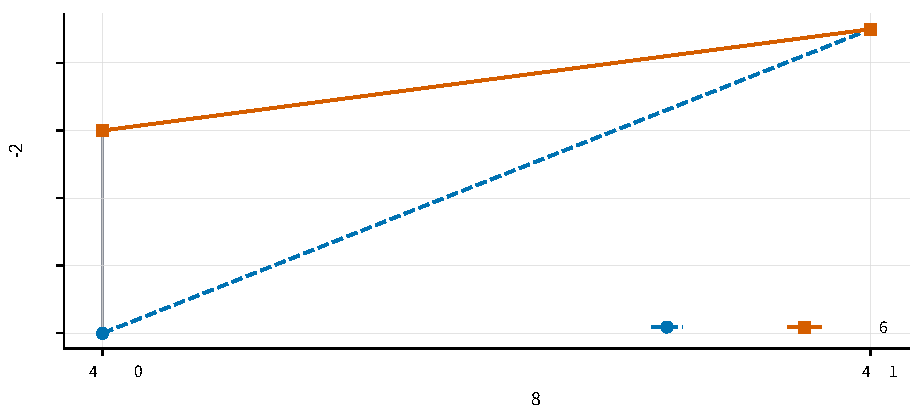
\includegraphics[width=0.93\linewidth]{figures/allocation-comparison.pdf}
  \caption{两个完成合成实例的目标值。竖线表示同一实例内两法的数值差，不是误差区间。
  \texttt{known-gap} 中穷举值高 $6$ value；\texttt{known-tie} 中两法同为 $21$ value。}
  \label{fig:comparison}
\end{figure}

为同时呈现数值、描述性差距和运行覆盖，图~\ref{fig:diagnostics} 使用三面板布局。
相对差距定义为 $(V_E-V_G)/V_E$，只用于解释单个已完成实例；状态面板把故意失败保留为醒目的独立单元。

\begin{figure}[H]
  \centering
  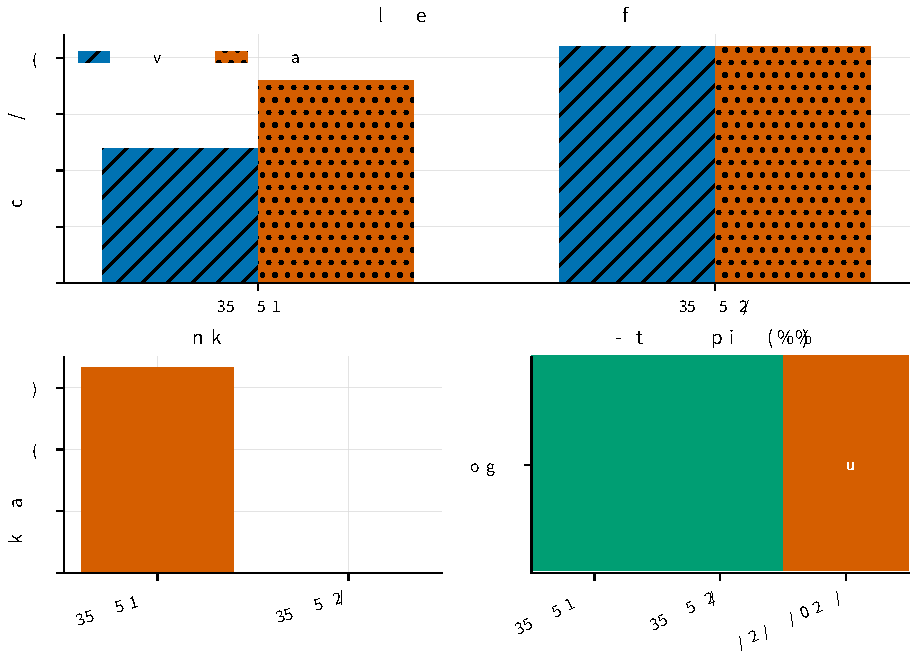
\includegraphics[width=0.98\linewidth]{figures/allocation-diagnostics.pdf}
  \caption{合成运行诊断。(a) 原始完整观测；(b) 相对穷举值的描述性差距；
  (c) 三个计划实例的状态。状态矩阵作为密集 artist 选择性栅格化，其余线条和文字保留为矢量。}
  \label{fig:diagnostics}
\end{figure}
